\documentclass[11pt,usenames,dvipsnames]{article}
\usepackage{lineno}
\usepackage{graphicx}
\usepackage[left=3cm, right=3cm, top=2cm]{geometry}
\usepackage{float}
\usepackage{caption}
\usepackage[round]{natbib}
\usepackage{pgfgantt}
\usepackage{amsmath}
\usepackage{booktabs}
\usepackage{amsfonts}
\usepackage[hidelinks]{hyperref} % for underscores in bibtex
\bibliographystyle{plainnat}
\captionsetup[table]{skip=12pt}
\linespread{1.3}
\setlength{\parskip}{2em}
\newcommand{\Lagr}{\mathcal{L}}
\newcommand{\lagr}{\mathcal{l}}
\DeclareMathOperator\erf{erf}
\begin{document}
\begin{titlepage}
\begin{center}
	\large{MSC. Computational Methods in Ecology and Evolution }\\
	\textbf{Thesis}\\[0cm]
	\huge{\line(1,0){380}\\
		Examining foraging distance distributions of the Western Honeybee, \textit{Apis mellifera}: A comparison between rural and urban environments\\
	\line(1,0){380}}\\[2cm]
\end{center}


\begin{minipage}[t]{0.5\textwidth}
\begin{flushleft}
	\Large{\textbf{Author}}\\
	\large{ Joseph Palmer\\
		CID: 01613406}\\
	joseph.palmer18@imperial.ac.uk\\[1cm]	
\end{flushleft}
\end{minipage}
\begin{minipage}[t]{0.5\textwidth}
\begin{flushright}
	\Large{\textbf{Supervisors}}\\
	\large{ Professor Vincent A.A. Jansen}\\
	Vincent.Jansen@rhul.ac.uk\\
	\large{Dr Elli Leadbeater}\\
	Elli.Leadbeater@rhul.ac.uk\\
	\large{Dr Richard J. Gill}\\
	r.gill@imperial.ac.uk
\end{flushright}
\end{minipage}

\vspace{1cm}
\begin{center}
	\large{\textbf{Imperial College London }}\\[0.2cm]
	\large{\textit{Department of Life Sciences, Imperial College London,}\\
		\textit{Ascot, Berkshire, SL5 7PY, United Kingdom}}\\[0.5cm]
	
	\large{\textbf{Royal Holloway University of London }}\\[0.2cm]
	\large{\textit{School of Biological sciences, Royal Holloway University of London,\\
			Egham Hill, Egham, Surrey, TW20 0EX, United Kingdom}}\\[0.5cm]
	\textbf{Word count:} 100 [replace]\\[0.5cm]
	\textbf{August 2019}
\end{center}

\end{titlepage}
\newpage
\tableofcontents
\newpage


\section{Introduction}

The western honey bee (\textit{Apis mellifera}) is among the most important pollinators for both natural and agricultural ecosystems \citep{Albrecht2018}. With a growing human population, the need for pollinators is arguably higher than ever before yet many pollinator species are in decline \citep{Powney2019}. Despite substantial research into pollinator behaviour their movement patterns remain largely unknown. With increases in urban and agri-rural landscapes, improving our understanding of pollinator movement in different environments is key to developing more effective argi-rural and urban management strategies.  

Whilst much attention has been given to mechanisms explaining movement patterns of certain pollinator species, there lacks a general consensus for movement as a whole \citep{Mueller2008,Nathan2008}. This is often an issue of practicality given the volume of pollinating species and the difficulty in collaborating multi-species studies. Studies of single species can illuminate underlying mechanisms, however, mechanistic approaches can often lead to more specific outcomes and potentially neglect more general processes common across species. To capture core underlying features of movement it has been argued that studies should take a more statistical approach to describe movements \Citep{VanMoorter2013}. 

Movement patterns are often described according to their biological purpose \citep{Fryxell2008}. For example, migratory movement is classified differently to foraging movement and mate search. This difference in biological mechanisms is mirrored by variations in scale, however, movement scales also differ within processes. \cite{Petrovskii2011} identified variations in individual walking behaviour of black bean aphids occurred at multiple scales, demonstrating that the concatenation of individual diffusive movements gives a super-diffusive signature at the population level. The authors attributed these differences in scale to variations in body size and leg length, highlighting the use of statistical methods to identify otherwise hidden physiological mechanisms.

Given the importance of scale in explaining animal movements this study seeks to identify to what extent honey bee foraging distances can be described as \textit{scale free}. Honey bees live in highly advanced eusocial colonies with overlapping generations and division of labour. As the colony functions as a single reproductive unit, worker bees have the shared task of optimising foraging effort so the colony can grow \citep{Samuelson2017}. With a typical colony size of 30,000 individuals, in temperate environments a typical colony must collect around 120 Kg of nectar and 20 Kg of pollen \citep{Seeley1995}. Consequentially, the representative foraging area of a colony is estimated at around 100 Km\textsuperscript{2} with 95\% of foraging trips occurring within 6 Km of the hive \citep{Samuelson2017}. In order to assist with resource acquisition, honey bees employ the waggle dance to convey information regarding the location of resources to nest mates. This offers us a unique window into the foraging behaviour of the colony as a whole and allows us to assess movement at different scales in this model central place forager. 

The focus on scale in animal movement research has long centred around diffusive and super-diffusive properties. Since Mandelbrot's suggestion of fractal properties in animal movement there has been increased attention to identify evidence of scale-free movement \citep{Harris2012,Ariel2015,Humphries2010,Baronchelli2013,Boyer,Ramos-Fernandez2004,Sims2008,Viswanathan1999}. Scale free movement is composed of multiple short flights interspersed with decreasingly probable longer flights (figure 1). The resulting distributions are characterised by a heavy tailed distribution and are classed as scale free as they have no characteristic scale \citep{Reynolds2018}. On double log axis the distribution shows a straight line, indicative of fractal processes. This theory was given mechanistic support by \cite{Shlesinger1986} in their recognition that Levi flights can provide an advantage for searching due to the reduced revisitation rates for previously explored areas. Consequentially, Levi flights are widely considered to represent an optimal searching strategy \citep{Viswanathan1999,Humphries2014}. However, the exact conditions that favour such a strategy, as well as whether or not Levi flights represent an emergent or evolved characteristic are debated \citep{Wosniack2017,Pyke2015,Kolzsch2015,DeJager2013}.  

\begin{figure}[H]
	\centering
	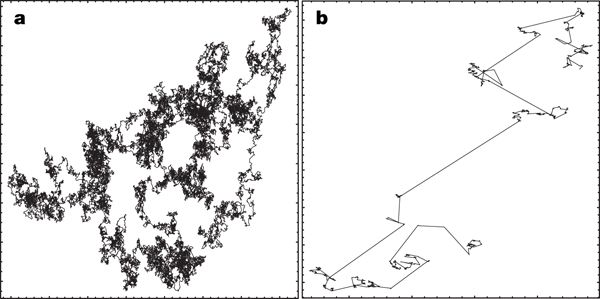
\includegraphics[scale=0.7]{LeviFlight.jpg}
	\caption{\textbf{a}) Brownian motion with equal contribution of step length to the average, \textbf{b}) Levi flight ($\gamma = 2$) with increased frequency of longer steps. Taken from \cite{Barthelemy2008}.}
\end{figure}

With the explosion in publications investigating movement distributions has come the shift from the binary Brownian motion Vs Levy flight debate to one that includes composite random walks \citep{Petrovskii2011,Sakamoto2017,Gautestad2012}. Composite random walks are identified as a middle point between Brownian motion and Levi flights. The statistical rational behind this is based upon scale, with a single exponential representing as a single scale and Levi flights being scale free. Consequentially, composite random walks are defined as a concatenation of exponentials, where by each exponential represents a given scale. Studies such as \cite{Sakamoto2017} and \cite{Zhao2016} have identified composite random walks better explained livestock movements than simple Brownian motion or Levi flights. 

The mechanistic rational behind these composite random walks is that they divide movement into separate groups, such as an intensive phase associated with moving around a small area and a relaxed phase characterised by movement between patches \citep{Auger-Methe2015}. This rational follows the classification of movement by purpose discussed earlier but whilst these methods provide an intermediate between Brownian motion and scale free movement, the number of exponentials used to identify the number of scales acting in the data are relatively low, often less than 4 \citep{Sakamoto2017,Zhao2016}. Given the suggestion by \cite{Petrovskii2011} that individuals move at different scales due to physiological differences, it is possible that limiting the number of exponentials in a composite random walk underestimates the number of scales potentially acting in a population. 

In order to fully analyse movement in terms of scale, we propose a new method which extends the work of \cite{Petrovskii2011} to a sum of $n$ exponentials. In doing so, the relative contributions of movements at different scales can be identified by weighting each exponential in the sum. This permits the identification of the amount of movement at a given scale without limiting the number of scales under consideration. This approach, theoretically at least, produces a more fine grained view of movements in terms of scale. As this method is centred around the use of an exponential function it is prudent to also compare the fits against other distributions. For this reason we also fit four distributions with different tail properties: the half-normal, log-normal, exponential and gamma distributions. By combining methods to identify contributions of different scales with other functions this study aims to provide a phenomenological profile of honey bee foraging in an agri-rural and urban landscape.

Whilst eves dropping on the waggle dance offers distinct advantages over other methods of evaluating foraging behaviour, there are limitations which dictate the study perspective. As the information gives us a vector of distance and direction we can pin point where the individual is telling other nest mates to visit, thus gaining only the information the bees have access to. This approach is free of the costs associated with other methods, such as with harmonic radar tracking which requires the subject be fit with a receiver device that could alter behaviour \citep{Oneal2004}. The limitations of using only waggle dance data, however, is that the information yielded does not provide any information on the mechanisms of searching, it only shows us where the colony is foraging. This rules out the ability to compare searching behaviour from individual flight lengths and so omits some aspects of forager movement.

Whilst the limitations of waggle dance data rules out comparing flight lengths within and between environments, the distance information can still be analysed to identify movement patterns of the colony. A similar approach is used in seed dispersal research \citep{Bullock2017}. In order to identify how plant seeds disperse, distance is used to form a dispersal kernel which can then be analysed statistically to identify underlying patterns between species. In taking this approach, distance data decoded from waggle dance observations is used to create a foraging kernel. Distances derived from waggle dance data have long been used as a proxy for forage availability in the local environment \citep{Visscher1982, Waddington1994, Couvillon2014, Couvillon2015}. Consequentially, by statistically describing this distribution in terms of scale we can identify how the colony as a whole utilises resources within the local environment and phenomenologically describe movement patterns.

\section{Methods}

\subsection{Data collection}
Foraging distances were collected by decoding waggle dance observations from honey bees in two sites, one in an agri-rural setting the other in an urban green space. The hives were set up as two three-frame observation hives of standard size in order to record waggle dances. Recordings took place for between two and four hours twice a month from April to September 2017. Waggle dance observations were collected and converted to longitude and latitude coordinates by Ash Samuelson as part of their PhD research with Royal Holloway University of London, under the supervision of Dr Ellie Leadbeater and Dr Richard Gill.


\subsection{Calculation of distance from waggle dance observations}
Foraging distances were calculated as the euclidean distance between the hive and decoded waggle dance coordinates. This was done through equations ?, ? and ?, where a and b are the hive and destination latitudes respectively, c and d are the hive and destination longitudes and k is the conversion constant for kilometres, 6371.

% foraging distance equations from coordinates
\begin{equation}
x = f_{(abcd)} = \sin\left(\frac{b - a}{2}\right)^2\ +\ \cos(a)\ \cos(b) \sin\left(\frac{d - c}{2}\right)^2 
\end{equation}
\begin{equation}
y = 2\ \text{atan2}(\sqrt{x}, \sqrt{1 - x})
\end{equation}
\begin{equation}
D_e = K\ y
\end{equation}

\subsection{Distribution fitting}

In order to identify the most probable distributions explaining foraging distance, 4 distributions were chosen as candidates: Exponential, Gamma, Half-normal and Lognormal (equations ?, ?, ? and ? respectively). These distributions were chosen as they represent a sample of light, exponential and half-normal, and heavy, gamma and lognormal, tailed common distributions.

\begin{equation}
%exponential pdf
e^{-\lambda x}
\end{equation}
\begin{equation}
%exponential ccdf
1 - e^{-\lambda x}
\end{equation}
\begin{equation}
%Gamma pdf
\frac{1}{\Gamma(k)\theta^k}x^{k-1}e^{-\frac{x}{\theta}}
\end{equation}
\begin{equation}
%Gamma ccdf
1 - \frac{1}{\Gamma(k)}\gamma(k,\frac{x}{\theta})
\end{equation}
\begin{equation}
%halfnormal pdf
\frac{\sqrt{2}}{\sigma \sqrt{\pi}} \exp \left(-\frac{x^2}{2 \sigma^2}\right)
\end{equation}
\begin{equation}
%halfnormal ccdf
\erf\left(\frac{x}{\sigma \sqrt{2}}\right)
\end{equation}
\begin{equation}
%lognormal pdf
\frac{1}{x \sigma \sqrt{2 \pi}}\ e^{- \frac{(\ln\ x - \mu)^2}{2\sigma^2}}
\end{equation}
\begin{equation}
%lognormal ccdf
\frac{1}{2} + \frac{1}{2}\ \erf\left[\frac{\ln\ x - \mu}{\sqrt{2 \sigma}}\right]
\end{equation}

To determine the parameters which best fit the distributions to the data we used maximum likelihood. This was conducted in Python using the Scipy package \textit{minimize} and the Sequential Least Squares Programming (SLSQP) method. The function minimises an objective function through gradient decent. Consequentially, we provided the method with the negative log-likelihood equations for each distribution in order to identify the parameters producing the maximum log-likelihood estimate (see supplementary equations ?, ?, ? and ?). Once the parameters with the highest likelihood are identified we fit the model to the complimentary cumulative distribution frequency (CCDF). This was chosen over the probability density function (PDF) as the probability of obtaining an exact value is 0, where as the CCDF allows us to view the probability of obtaining a value greater than or equal to a particular value (see supplementary equations ?, ?, ? and ?). 


\subsection{Sum of exponentials procedure}

The sum of exponentials (SumExp) procedure is composed of $n$ exponential functions (equation ?) summed together, each constrained by a weighting factor (equation ?, subject to equations ? and ?). The parameters of the model are $\lambda$ and $\psi$, where $\lambda$ is the rate component of the exponential and $\psi$ is the weighting factor which influences the relative contribution of an exponential with a given rate in the sum. $\lambda$ values are restricted to only positive real numbers (equation ?) and both individual $\psi$ and the combined sum of $\psi$ values must be greater than or equal to 0 and less than or equal to 1 (equation ?).

\begin{equation}
%single exponential equation
\lambda e^{-\lambda x}
\end{equation}
\begin{equation}
% sum of exponentials equation
f(x) = \sum_{i=1}^{n-1} \psi_i \lambda_i e^{-\lambda_i x} + \left(1 - \sum_{i=1}^{n-1}\psi_i\right) \lambda_n e^{-\lambda_n x}
\end{equation}
subject to (eq ?, ? \& ?)
\begin{equation}
% constraints on individual psi
0\leq \psi_i \leq 1
\end{equation}
\begin{equation}
% constraints on sum of psi
0\leq \sum_{i=1}^{n-1}\psi_i \leq 1
\end{equation}
\begin{equation}
% constraints on individual lambda
\lambda = \mathbb{R}^+
\end{equation}

\subsection{Numerical optimisation}

In order to identify the most probable parameter values for the SumExp model we used numerical optimisation to estimate the parameters with maximum likelihood. The procedure for doing this is to take the product of Sumexp over the number of observations (equation ?) and find the peak in the resulting likelihood curve. For easier computation the log-likelihood is used herein (equation ?). The analysis was conducted in Python using the scipy.optimize package \textit{minimize} (ref) and the Sequential Least Squares Programming (SLSQP) routine (ref) to identify the minima of the negative log-likelihood function. The SLSQP method uses gradient decent to scale the likelihood curve until the model derivative is within a given tolerance of 0. As such, the gradient function of partial derivatives (equation ?) is provided to improve convergence.

\begin{equation}
%likelihood equation for SumExp
\Lagr_{(\psi|x)} = \prod_{i=1}^{n} f(x)
\end{equation} 
\begin{equation}
%loglikelihodd equation for SumExp
\ell_{(\psi|x)} = \sum_{i=1}^{n} \ln f(x)
\end{equation} 
\begin{equation}
% gradient function of partial derivitives of SumExp. 
\nabla h(x) = \begin{bmatrix} -\sum_{i=1}^{n} [\frac{\lambda_0 e^{-\lambda_0 x_i}}{f(x_i)} - \frac{\lambda_n e^{-\lambda_n x_i}}{f(x_i)}] \\
... \\
... \\
-\sum_{i=1}^{n} [\frac{\lambda_{n-1} e^{-\lambda_{n-1} x_i}}{f(x_i)} - \frac{\lambda_n e^{-\lambda_n x_i}}{f(x_i)}] \\
\end{bmatrix}
\end{equation}

The optimisation procedure used involves selecting multiple rates evenly spaced over a given interval to create a SumExp of a given size. These rates are then fixed in the model but the weights are left as free parameters within their bounds and constraints. If the rates are free in the model along with the weights then the procedure would identify the most probable sum of exponentials explaining the data. Instead, by keeping the rates fixed we allow the weights to act as switches that limit the contribution of an associated rate. By varying the upper and lower bounds as well as the number of rates (resolution) the procedure can be used to explore the data in terms of scale and aid the development of more parsimonious models. 

\subsection{Experimental error}
The distributions of data in our study showed distances bellow 1Km, which corresponds to approximately less than 1 second of waggle dance duration. Whilst it is entirely plausible such short dances are representative of foraging locations, it is important to consider possible measurement errors influencing the data. To consider this we present results of both the full data set and the data excluding points bellow 1Km. 

\section{Results}

\noindent
\subsection{Simulated data}

\subsubsection{Single exponential}
In order to test if the numerical method can identify the sum of exponentials with the most likely parameter estimates, we tested data sampled from a single exponential with $\lambda = 1.8$. Sampling 1,000 data points we calculated the analytical rate parameter, derived as the reciprocal of the data mean, is 1.82 with an associated maximum likelihood estimate (MLE) of -401.28. The sum of exponentials method identified a distribution with a single dominant cluster of 2 peaks at rates 1.83 and 1.85 and associated weights of 0.93 and 0.059; explaining 99\% of the observations. The remaining 1\% is explained by a peak at $\lambda = 0.86$ (figure ?). The associated MLE is -401.26. Therefore, although the likelihood is slightly improved, the added parameters indicate the single exponential is the more parsimonious model.

\begin{figure}[H]
	\centering
	\includegraphics[scale=1]{../Results/Plots/SyntheticData_1exp.pdf}
	\caption{Scale spectrum of linearly selected rates for data sampled from a single exponential with $\lambda = 1.8$.}
\end{figure}


\subsubsection{Multiple exponentials}

\noindent
\textbf{Equal weighting (50/50)}

In order to test if the method can identify data derived from processes operating at two different scales, we sampled data points from a sum of two exponentials with rates 1.8 and 4.4 and equal weights. With a sample size of 1,000 the method identified five rates in 3 district clusters with $\lambda$ approximately 1.26, 2.68 and 6.49 and associated $\psi$ of approximately 0.11, 0.78 and 0.11 (Table ?, figure ?). With 10,000 observations the rates form two main clusters around rates 1.87 and 4.6 with associated $\psi$ values of 0.55 and 0.42. At 100,000 observations the rate peaks appear close to the actual input values with $\psi$ matching the input weightings (table ?). 

\begin{table}[H]
	\centering
	\caption{Numerically optimised rates ($\lambda$) and weights ($\psi$) with data sampled from $n$ observations of a sum of two exponentials with $\lambda = 1.8,\ 4.4$ and $\psi = 0.5$.}
	\begin{tabular}{rrr}
\toprule
    $n$ &  $\lambda$ &    $\psi$ \\
\midrule
   1000 &       1.24 &  0.003290 \\
   1000 &       1.30 &  0.111582 \\
   1000 &       2.68 &  0.777452 \\
   1000 &       6.46 &  0.002152 \\
   1000 &       6.52 &  0.105525 \\
  10000 &       1.00 &  0.003992 \\
  10000 &       1.84 &  0.144445 \\
  10000 &       1.90 &  0.416288 \\
  10000 &       4.60 &  0.415916 \\
  10000 &       9.94 &  0.019359 \\
 100000 &       1.78 &  0.280559 \\
 100000 &       1.84 &  0.218817 \\
 100000 &       4.36 &  0.304631 \\
 100000 &       4.42 &  0.195990 \\
\bottomrule
\end{tabular}

\end{table}


\begin{figure}[H]
	\centering
	\includegraphics[scale=1]{../Results/Plots/SyntheticData_2exp1844.pdf}
	\caption{Scale spectrum of linearly selected rates for data sampled from a sum of two exponentials with $\lambda = 1.8,\ 4.4$ and $\psi = 0.5$. Upper bound $= 10$, lower bound $= 0$, resolution $= 150$ \textbf{A}) $n = 1,000$, \textbf{B}) $n = 10,000$,  \textbf{C}) $n = 100,000$.}
\end{figure}

\noindent
\textbf{Unequal weighting (70/30)}

Using the same parameters as above but with unequal weightings of 0.3 and 0.7 for rates 1.8 and 4.4 respectively, we again tested how the method performs with different data sizes. With a data size of 1,000 the method identified two main peaks around 1.6 and 3.85 with corresponding $\psi$ values of 0.18 and 0.73. For 10,000 observations the main peaks are at 2.02 and 4.09 with associated $\psi$ of 0.33 and 0.6 with the remainder at rates 1.0 and 9.94. With 100,000 observations the peaks lie at 1.71 and 4.39, just as with equal weighting (figure ?, table?) but the weighting is 0.3 and 0.7 respectively (figure?, table?). Overall, these results indicate the method is able to identify the appropriate weighting ($\psi$) even at low data sizes, but the convergence towards the 'true' input values increases with data size.

\begin{table}[H]
	\centering
	\caption{Numerically optimised rates ($\lambda$) and weights ($\psi$) with data sampled from $n$ observations of a sum of two exponentials with $\lambda = 1.8,\ 4.4$ and $\psi = 0.5$.}
	\begin{tabular}{rrr}
\toprule
    $n$ &  $\lambda$ &    $\psi$ \\
\midrule
   1000 &       1.54 &  0.047849 \\
   1000 &       1.60 &  0.129053 \\
   1000 &       3.82 &  0.352723 \\
   1000 &       3.88 &  0.382955 \\
   1000 &       3.94 &  0.087421 \\
  10000 &       1.00 &  0.008807 \\
  10000 &       2.02 &  0.331551 \\
  10000 &       4.06 &  0.238486 \\
  10000 &       4.12 &  0.360444 \\
  10000 &       9.94 &  0.060711 \\
 100000 &       1.78 &  0.248727 \\
 100000 &       1.84 &  0.048693 \\
 100000 &       4.36 &  0.543943 \\
 100000 &       4.42 &  0.155287 \\
 100000 &       9.94 &  0.003350 \\
\bottomrule
\end{tabular}

\end{table}


\begin{figure}[H]
	\centering
	\includegraphics[scale=1]{../Results/Plots/SyntheticData_2exp1844_73.pdf}
	\caption{Scale spectrum of linearly selected rates for data sampled from a sum of two exponentials with $\lambda = 1.8,\ 4.4$ and $\psi = 0.5$. Upper bound $= 10$, lower bound $= 0$, resolution $= 150$ \textbf{A}) $n = 1,000$, \textbf{B}) $n = 10,000$,  \textbf{C}) $n = 100,000$.}
\end{figure}

\noindent
\textbf{Five rate sum of exponentials}

In order to test how the method responds to processes operating at multiple scales we sampled data from a five rate sum of exponential. As the previous results indicate the method can over fit to data, we used very different rates to represent processes with multiple scales scanning several orders of magnitude. The rates used are 1.8, 4.4, 7.5, 12.5 and 16.7 with equal weightings of 0.2. With a sample size of 1,000 the method identified 4 peaks with rates of 1.5, 2.74, 9.65 and 22.5 and corresponding $\psi$ of 0.05, 0.29, 0.38 and 0.28 (table ?, figure ?). 10,000 observations returned 3 main peaks at rates 2.15, 4.89 and 12.6 with corresponding $\psi$ values of 0.24, 0.23, and 0.48, with the remainder located at two other peaks of 1.0 and 29.9. With 100,000 observations the method identified four main peaks at rates 1.79, 4.3, 7.34 and 15.43 with corresponding $\psi$ values of 0.21, 0.14, 0.29 and 0.35 (table ? figure ?). 

\begin{table}[H]
	\centering
	\caption{Numerically optimised rates ($\lambda$) and weights ($\psi$) with data sampled from $n$ observations of a sum of five exponentials with $\lambda = 1.8,\ 4.4,\ 7.5,\ 12.5,\ 16.7$ and $\psi = 0.2$.}
	\begin{tabular}{rrr}
\toprule
    $n$ &  $\lambda$ &    $\psi$ \\
\midrule
   1000 &   1.497143 &  0.050242 \\
   1000 &   2.740000 &  0.285434 \\
   1000 &   9.617143 &  0.128375 \\
   1000 &   9.700000 &  0.195719 \\
   1000 &   9.782857 &  0.181994 \\
   1000 &   9.865714 &  0.094545 \\
   1000 &  22.377143 &  0.003371 \\
   1000 &  22.460000 &  0.020353 \\
   1000 &  22.542857 &  0.019953 \\
   1000 &  22.625714 &  0.015760 \\
   1000 &  22.708571 &  0.004230 \\
  10000 &   1.000000 &  0.009865 \\
  10000 &   2.077143 &  0.045273 \\
  10000 &   2.160000 &  0.194265 \\
  10000 &   4.894286 &  0.234190 \\
  10000 &  12.517143 &  0.080454 \\
  10000 &  12.600000 &  0.216137 \\
  10000 &  12.682857 &  0.188127 \\
  10000 &  29.917143 &  0.031690 \\
 100000 &   1.745714 &  0.006408 \\
 100000 &   1.828571 &  0.203963 \\
 100000 &   4.314286 &  0.126473 \\
 100000 &   4.397143 &  0.017868 \\
 100000 &   7.214286 &  0.001503 \\
 100000 &   7.297143 &  0.146539 \\
 100000 &   7.380000 &  0.143362 \\
 100000 &  15.334286 &  0.050094 \\
 100000 &  15.417143 &  0.136866 \\
 100000 &  15.500000 &  0.132326 \\
 100000 &  15.582857 &  0.034596 \\
\bottomrule
\end{tabular}

\end{table}
\begin{figure}[H]
	\centering
	\includegraphics[scale=1]{../Results/Plots/SyntheticData_2exp1844_5.pdf}
	\caption{Scale spectrum of linearly selected rates for data sampled from a sum of five exponentials with $\lambda = 1.8,\ 4.4,\ 7.5,\ 12.5,\ 16.7$ and $\psi = 0.2$. Upper bound $= 30$, lower bound $= 1$, resolution $= 350$. \textbf{A}) $n = 1,000$, \textbf{B}) $n = 10,000$,  \textbf{C}) $n = 100,000$.}
\end{figure}

What is notable here is that the method was unable to identify the input rates and appropriate weights at any of the data sizes tested. Although they converged towards to the true values as sample size was increased, the procedure omitted the rate 12.5. This indicates the method struggles to identify process occurring at more than 3 or 4 scales without very large data sets, possibly due to overlaps in parameter space (figure ?).

\begin{figure}[H]
	\centering
	\includegraphics[scale=1]{../Results/Plots/SyntheticData_Hist_5.pdf}
	\caption{Overlapping histograms of data sampled from exponentials with different rates. \textbf{A}) $\lambda = 1.8, 4.4$, \textbf{B}) $\lambda = 1.8, 4.4, 7.5$, \textbf{C}) $\lambda = 1.8, 4.4, 7.5, 12.5$, \textbf{D}) $\lambda = 1.8, 4.4, 7.5, 12.5, 16.7$.}
\end{figure}


\subsection{Analysis of foraging distance}

The agri-rural data consists of 193 observations ranging from 0.016 to 5.17Km with a mean of 1.29. The urban data consists of 221 observations ranging from 0.0006 to 3.18Km with a mean of 0.85. Combined these datasets consist of 414 observations ranging from 0.0006 to 5.17Km with a mean of 1.05.

\begin{figure}[H]
	\centering
	\includegraphics[scale=1]{../Results/Plots/DistributionHist.pdf}
	\caption{Histogram of agri-rural (\textbf{A}), urban (\textbf{B}) and combined (\textbf{C}) foraging distances.}
\end{figure}

With values bellow 1Km removed and the remaining data normalised by subtracting 1 from the distances, the agri-rural data consists of 107 observations ranging from 0.025 to 4.17Km with a mean of 0.85. The urban data consists of 81 observations ranging from 0.006 to 2.18Km with a mean of 0.53. Combined these datasets consist of 188 observations ranging from 0.0006 to 4.17Km with a mean of 0.71.

\begin{figure}[H]
	\centering
	\includegraphics[scale=1]{../Results/Plots/DistributionHist_1km.pdf}
	\caption{Histogram of agri-rural (\textbf{A}), urban (\textbf{B}) and combined (\textbf{C}) foraging distances above 1Km, normalised by subtracting 1Km from results.}
\end{figure}

In order to accommodate for the difference in distributions between these two data sets, foraging distances were compared using a bootstrapped hypothesis test. This was chosen as a non-parametric equivalent to the t-test as the data violates the condition of normality (figure ? histogram), whilst retaining a high degree of statistical power (ref on bootstrapping). For both the truncated and full data sets, foraging distance differed significantly between environments (Non-parametric bootstrap test: simulations = 10,000. full data: agri-rural mean = 1.29, urban mean 0.85, degrees of freedom = 192 and 220, t = 5.70, p $\le$ 0.001; truncated data: agri-rural mean = 0.85, urban mean 0.53, degrees of freedom = 106 and 80, t = 3.34, p < 0.01) (figure ?). 

\begin{figure}[H]
	\centering
	\includegraphics[scale=0.9]{../Results/Plots/DistDiff.pdf}
	\caption{Comparison of agri-rural and urban mean foraging distances. With both datasets foraging distance is significantly different between environments (Non-parametric bootstrap test: simulations = 10,000) \textbf{A}) Full data, agri-rural mean = 1.29, urban mean 0.85, degrees of freedom = 192 and 220, t = 5.70, p < 0.001. \textbf{B}) Truncated data, agri-rural mean = 0.85, urban mean 0.53, degrees of freedom = 106 and 80, t = 3.34, p $\le$ 0.01}
\end{figure}

\subsection{Fitting distributions using maximum likelihood}

\subsubsection{Full data}
In order to determine the distribution which best describes the data, maximum likelihood methods were used to fit a number of candidate distributions. Each distribution was fit to the urban and agri-rural data and the fit assessed using the Akaike information criterion (AIC) and associated Akaike weights (AICw). For the rural data the most parsimonious model is the gamma distribution (table ?) with an AIC score seven points lower than the next best fitting model, the half-normal distribution. Using Akaike weights we can determine the probability that a given model is the best model of our candidate set. By dividing the AICw of the best model by that of the next best candidate (0.978/0.0233), the Gamma distribution is approximately 41.9 times more likely to be the best model in terms of the Kullback–Leibler discrepancy than the half-normal model.

For the urban data, the best fitting model is the half-normal distribution with an AIC score 14 points lower than the next best fitting model, the gamma distribution (table ?, figure ?). The interpretation of Akaike weights indicates the half-normal is approximately 1225.5 times more likely to represent the best model in terms of the Kullback–Leibler discrepancy than the Gamma distribution.

For the agri-rural and urban foraging data combined, the best fitting model is the half-normal with an AIC score 10 points lower than the next best fitting model, the gamma distribution (table ?, figure ?). The interpretation of Akaike weights indicates the half-normal is approximately 196.1 times more likely to represent the best model in terms of the Kullback–Leibler discrepancy than the Gamma distribution.

\begin{table}[H]
	\centering
	\caption{AIC and weighted AIC scores for distributions fit using maximum likelihood to Agri-rural foraging distances.}
	\begin{tabular}{llrr}
\toprule
Distribution &      MLE &         AIC &          AICw \\
\midrule
       Gamma & -222.258 &  448.516283 &  9.766669e-01 \\
 Half-normal & -226.992 &  455.984833 &  2.333305e-02 \\
 Exponential & -242.106 &  486.211336 &  6.373377e-09 \\
   Lognormal & -244.337 &  492.674635 &  2.516994e-10 \\
\bottomrule
\end{tabular}

\end{table}
\begin{table}[H]
	\centering
	\caption{AIC and weighted AIC scores for distributions fit using maximum likelihood to urban foraging distances.}
	\begin{tabular}{llrr}
\toprule
Distribution &      MLE &         AIC &          AICw \\
\midrule
 Half-normal & -174.376 &  350.751452 &  9.991404e-01 \\
       Gamma & -180.487 &  364.973596 &  8.153183e-04 \\
 Exponential & -184.401 &  370.801177 &  4.424703e-05 \\
   Lognormal & -215.753 &  435.506022 &  3.939176e-19 \\
\bottomrule
\end{tabular}

\end{table}
\begin{table}[H]
	\centering
	\caption{AIC and weighted AIC scores for distributions fit using maximum likelihood to combined argi-rural and urban foraging distances.}
	\begin{tabular}{llrr}
\toprule
Distribution &      MLE &         AIC &          AICw \\
\midrule
 Half-normal & -416.694 &  835.388612 &  9.949263e-01 \\
       Gamma & -420.973 &  845.945810 &  5.073695e-03 \\
 Exponential & -435.614 &  873.228880 &  6.037832e-09 \\
   Lognormal &  -483.13 &  970.260184 &  5.138081e-30 \\
\bottomrule
\end{tabular}

\end{table}

\begin{figure}[H]
	\centering
	\includegraphics[scale=1]{../Results/Plots/RuralDistributionFit.pdf}
	\caption{Complementary Cumulative Distribution Frequency (CCDF) of agri-rural foraging distances with fitted model lines. A) Exponential, B) Gamma, C) Half-normal, D) Lognormal.}
\end{figure}

\begin{figure}[H]
	\centering
	\includegraphics[scale=1]{../Results/Plots/UrbanDistributionFit.pdf}
	\caption{Complementary Cumulative Distribution Frequency (CCDF) of urban foraging distances with fitted model lines. A) Exponential, B) Gamma, C) Half-normal, D) Lognormal.}
\end{figure}

\begin{figure}[H]
	\centering
	\includegraphics[scale=1]{../Results/Plots/AllDistributionFit.pdf}
	\caption{Complementary Cumulative Distribution Frequency (CCDF) of combined agri-rural and urban foraging distances with fitted model lines. A) Exponential, B) Gamma, C) Half-normal, D) Lognormal.}
\end{figure}

\subsubsection{Truncated data}

\hspace{\parindent}
With distances lower than one Kilometre removed, and the remaining distances normalised by subtracting 1, the agri-rural data shows the best fitting model is the gamma. However the difference in AIC is less than 1 point to the next best fitting model, the exponential (table ?). A comparison of the weighted AIC scores suggests the gamma is approximately 1.4 times more likely to be most parsimonious model than the exponential (table ?).

In contrast, the urban data shows the best model as the exponential, almost 2 AIC points lower than the next best fitting model, the gamma distribution (table ?). The comparison of AIC weights indicates the exponential is approximately 2.5 times more likely to be the best model than the gamma (table ?).

For both the agri-rural and urban foraging distances combined, the best model was identified as the exponential, 2 AIC points lower than the next best fitting model, the gamma distribution (table ?). The comparison of AIC weights indicates the exponential is approximately 2.5 times more likely to be the best model than the gamma (table ?). 

\begin{table}[H]
	\centering
	\caption{AIC and weighted AIC scores for distributions fit using maximum likelihood to Agri-rural foraging data greater than 1Km.}
	\begin{tabular}{llrr}
\toprule
Distribution &      MLE &         AIC &      AICw \\
\midrule
       Gamma & -88.4953 &  180.990608 &  0.444697 \\
 Exponential & -89.8349 &  181.669702 &  0.316665 \\
   Lognormal & -89.1227 &  182.245326 &  0.237468 \\
 Half-normal & -95.4361 &  192.872228 &  0.001170 \\
\bottomrule
\end{tabular}

\end{table}
\begin{table}[H]
	\centering
	\caption{AIC and weighted AIC scores for distributions fit using maximum likelihood to urban foraging data greater than 1Km.}
	\begin{tabular}{llrr}
\toprule
Distribution &      MLE &        AIC &      AICw \\
\midrule
 Exponential &  -29.446 &  60.891934 &  0.699804 \\
       Gamma & -29.3618 &  62.723513 &  0.280062 \\
 Half-normal & -32.9953 &  67.990502 &  0.020116 \\
   Lognormal &  -39.024 &  82.048053 &  0.000018 \\
\bottomrule
\end{tabular}

\end{table}
\begin{table}[H]
	\centering
	\caption{AIC and weighted AIC scores for distributions fit using maximum likelihood to combined argi-rural and urban foraging distances greater than 1Km.}
	\begin{tabular}{llrr}
\toprule
Distribution &      MLE &         AIC &          AICw \\
\midrule
 Exponential & -124.347 &  250.693054 &  7.134821e-01 \\
       Gamma & -124.259 &  252.517781 &  2.865158e-01 \\
   Lognormal & -136.396 &  276.792210 &  1.534700e-06 \\
 Half-normal & -138.436 &  278.871001 &  5.427747e-07 \\
\bottomrule
\end{tabular}

\end{table}

\begin{figure}[H]
	\centering
	\includegraphics[scale=1]{../Results/Plots/RuralDistributionFit_1km.pdf}
	\caption{Complementary Cumulative Distribution Frequency (CCDF) of agri-rural foraging distances over 1Km with fitted model lines. A) Exponential, B) Gamma, C) Half-normal, D) Lognormal.}
\end{figure}
\begin{figure}[H]
	\centering
	\includegraphics[scale=1]{../Results/Plots/UrbanDistributionFit_1km.pdf}
	\caption{Complementary Cumulative Distribution Frequency (CCDF) of urban foraging distances over 1Km with fitted model lines. A) Exponential, B) Gamma, C) Half-normal, D) Lognormal.}
\end{figure}
\begin{figure}[H]
	\centering
	\includegraphics[scale=1]{../Results/Plots/AllDistributionFit_1km.pdf}
	\caption{Complementary Cumulative Distribution Frequency (CCDF) of combined agri-rural and urban foraging distances over 1Km with fitted model lines. A) Exponential, B) Gamma, C) Half-normal, D) Lognormal.}
\end{figure}

\subsection{Sum of exponential fitting}

\subsubsection{Full data}

For the agri-rural data, using variations of fixed rates between 0 and 100, the method identified a single exponential with $\lambda = 0.77$ most likely contributed to the data. This matches the analytically derived single exponential rate value (figure ?, table ?). For the urban data a single peak is also identified around 1.18 again matching the analytical MLE for a single exponential (figure ?, table ?). When the data from each site is combined, the method identified a single peak at $\lambda = 0.94$ explained the data best, within 0.01 of the analytical MLE of the combined data (table ?, figure ?). 

\begin{table}[H]
	\centering
	\caption{Estimated rate ($\lambda$) and weight ($\psi$) sum of exponential parameters for agri-rural and urban foraging distances. Analytical $\lambda$ derived from MLE of single exponential.}
	\begin{tabular}{lrrr}
\toprule
   Location &  $\lambda$ &    $\psi$ &  Analytical $\lambda$ \\
\midrule
 Agri-rural &   0.771429 &  0.916771 &              0.775356 \\
 Agri-rural &   0.777143 &  0.083229 &              0.775356 \\
      Urban &   1.171429 &  0.084733 &              1.180111 \\
      Urban &   1.177143 &  0.915253 &              1.180111 \\
   Combined &   0.948571 &  1.000000 &              0.949131 \\
\bottomrule
\end{tabular}

\end{table}


\begin{figure}[H]
	\centering
	\includegraphics[scale=1]{../Results/Plots/Sumexp_rural_full.pdf}
	\caption{\textbf{A}) Scale spectrum of agri-rural foraging distances. Single peak identified with $\lambda = 0.77$, upper bound $= 2$, lower bound $= 0$, resolution $= 350$. \textbf{B}) Complementary Cumulative Distribution Frequency (CCDF) of agri-rural foraging distances. Black line is data, blue line is sum of exponentials fit.}
\end{figure}

\begin{figure}[H]
	\centering
	\includegraphics[scale=1]{../Results/Plots/Sumexp_urban_full.pdf}
	\caption{\textbf{A}) Scale spectrum of urban foraging distances. Single peak identified with $\lambda = 1.18$, upper bound $= 2$, lower bound $= 0$, resolution $= 350$. \textbf{B}) Complementary Cumulative Distribution Frequency (CCDF) of urban foraging distances. Black line is data, blue line is sum of exponentials fit.}
\end{figure}

\begin{figure}[H]
	\centering
	\includegraphics[scale=1]{../Results/Plots/Sumexp_comb_full.pdf}
	\caption{\textbf{A}) Scale spectrum of combined agri-rural and urban foraging distances. Single peak identified with $\lambda = 0.94$, upper bound $= 4$, lower bound $= 0$, resolution $= 350$. \textbf{B}) Complementary Cumulative Distribution Frequency (CCDF) of urban foraging distances. Black line is data, blue line is sum of exponentials fit.}
\end{figure}


\subsubsection{Truncated data}

For the agri-rural foraging data over 1Km, using variations of fixed rates between 0 and 100, the method identified a single peak around $\lambda = 1.17$ most likely contributed to the data. This matches the analytically derived single exponential rate value (figure ?, table ?). For the urban foraging data over 1Km the method identified two peaks around rates 1.86 and 46.9. The peak around 1.86 is the dominant peak, explaining 97\% of the data with the remainder produced by the secondary peak. Consequentially, the second peak is small in figure ? (figure ?, table ?). The dominant peak is 0.03 larger than the analytical MLE of a single exponential for this data, 1.189. The associated likelihoods between the sum of exponentials and the single exponential is -29.081 and -29.446 respectively, however, this is not significantly different and indicates the single exponential is the more parsimonious model (Sum of exponentials $MLE = -29.08\ AIC = 76.2, AIC_w < 0.001$, single exponential $MLE = -29.46\ AIC = 60.9, AIC_w > 0.999$, table ?). 

Combined, the foraging data from both sites showed two peaks around rates 1.36 and 2.08, explaining 90\% and 10\% of the data respectively (table ?, figure ?). The likelihood for the sum of exponential and a single exponential is 0.02 higher than for the single exponential, however this is not significant indicating the single exponential is the more parsimonious model (SumExp $MLE = -124.33,\ AIC = 284.67,\ AIC_w < 0.001$, single exponential $MLE = -124.35,\ AIC = 250.69,\ AIC_w > 0.999$, table ?).

\begin{table}[H]
	\centering
	\caption{Estimated rate ($\lambda$) and weight ($\psi$) sum of exponential parameters for agri-rural, urban and combined foraging distances. Analytical $\lambda$ derived from MLE of single exponential.}
	\begin{tabular}{lrrr}
\toprule
   Location &  $\lambda$ &    $\psi$ &  Analytical $\lambda$ \\
\midrule
 Agri-rural &   1.154286 &  0.038405 &              1.174006 \\
 Agri-rural &   1.160000 &  0.158546 &              1.174006 \\
 Agri-rural &   1.165714 &  0.225814 &              1.174006 \\
 Agri-rural &   1.171429 &  0.241893 &              1.174006 \\
 Agri-rural &   1.177143 &  0.208409 &              1.174006 \\
 Agri-rural &   1.182857 &  0.126933 &              1.174006 \\
      Urban &   1.818182 &  0.913226 &              1.889797 \\
      Urban &   1.909091 &  0.055472 &              1.889797 \\
      Urban &  46.636364 &  0.002272 &              1.889797 \\
      Urban &  46.727273 &  0.003751 &              1.889797 \\
      Urban &  46.818182 &  0.004365 &              1.889797 \\
      Urban &  46.909091 &  0.004139 &              1.889797 \\
      Urban &  47.000000 &  0.004755 &              1.889797 \\
      Urban &  47.090909 &  0.007131 &              1.889797 \\
      Urban &  47.181818 &  0.004889 &              1.889797 \\
   Combined &   1.285714 &  0.008211 &              1.402957 \\
   Combined &   1.300000 &  0.067885 &              1.402957 \\
   Combined &   1.314286 &  0.106875 &              1.402957 \\
   Combined &   1.328571 &  0.128086 &              1.402957 \\
   Combined &   1.342857 &  0.134152 &              1.402957 \\
   Combined &   1.357143 &  0.127452 &              1.402957 \\
   Combined &   1.371429 &  0.110134 &              1.402957 \\
   Combined &   1.385714 &  0.087323 &              1.402957 \\
   Combined &   1.400000 &  0.063454 &              1.402957 \\
   Combined &   1.414286 &  0.047699 &              1.402957 \\
   Combined &   1.428571 &  0.024425 &              1.402957 \\
   Combined &   2.042857 &  0.006489 &              1.402957 \\
   Combined &   2.057143 &  0.014659 &              1.402957 \\
   Combined &   2.071429 &  0.019576 &              1.402957 \\
   Combined &   2.085714 &  0.020986 &              1.402957 \\
   Combined &   2.100000 &  0.018636 &              1.402957 \\
   Combined &   2.114286 &  0.012281 &              1.402957 \\
   Combined &   2.128571 &  0.001677 &              1.402957 \\
\bottomrule
\end{tabular}

\end{table}

\begin{table}[H]
	\centering
	\caption{Model statistics for urban foraging distances greater than 1Km.}
	\begin{tabular}{lrrr}
\toprule
  Model &        MLE &        AIC &      AICw \\
\midrule
    Exp & -29.445967 &  60.891934 &  0.999517 \\
 SumExp & -29.080624 &  76.161249 &  0.000483 \\
\bottomrule
\end{tabular}

\end{table}

\begin{table}[H]
	\centering
	\caption{Model statistics for combined agri-rural and urban foraging distances greater than 1Km.}
	\begin{tabular}{lrrr}
\toprule
  Model &         MLE &         AIC &          AICw \\
\midrule
    Exp & -124.346527 &  250.693054 &  1.000000e+00 \\
 SumExp & -124.334338 &  284.668675 &  4.190710e-08 \\
\bottomrule
\end{tabular}

\end{table}

\begin{figure}[H]
	\centering
	\includegraphics[scale=1]{../Results/Plots/Sumexp_rural_trun.pdf}
	\caption{\textbf{A}) Scale spectrum of agri-rural foraging distances. Single peak identified with $\lambda = 1.17$, upper bound $= 2$, lower bound $= 0$, resolution $= 350$. \textbf{B}) Complementary Cumulative Distribution Frequency (CCDF) of agri-rural foraging distances. Black line is data, blue line is sum of exponentials fit.}
\end{figure}

\begin{figure}[H]
	\centering
	\includegraphics[scale=1]{../Results/Plots/Sumexp_urban_trun.pdf}
	\caption{\textbf{A}) Scale spectrum of urban foraging distances. Two peaks identified around $\lambda = 1.86$ and $46.9$ with associated $\psi = 0.97$ and $0.03$, upper bound $= 50$, lower bound $= 0$, resolution $= 550$. \textbf{B}) Complementary Cumulative Distribution Frequency (CCDF) of urban foraging distances. Black line is data, blue line is sum of exponentials fit.}
\end{figure}

\begin{figure}[H]
	\centering
	\includegraphics[scale=1]{../Results/Plots/Sumexp_comb_trun.pdf}
	\caption{\textbf{A}) Scale spectrum of combined foraging distances from agri-rural and urban sites. Two peaks identified with $\lambda = 1.36$ and $2.08$ with associated $\psi = 0.9$ and $0.1$, upper bound $=5$, lower bound $= 0$, resolution $= 350$. \textbf{B}) Complementary Cumulative Distribution Frequency (CCDF) of combined foraging distances from agri-rural and urban sites. Black line is data, blue line is sum of exponentials fit.}
\end{figure}

\section{Discussion}

\subsection{Synthetic Data}
In order to build confidence in the results of this new method when applied to biological data it is important to demonstrate the method can retrieve known rates from synthetic data. By sampling data from a single exponential distribution we are able to test the desired switch behaviour of the weights. That the method identified a single rate explained almost all of the data, closely resembling the analytically derived rate indicates the weighting parameters function as desired. Although approximately 1\% of the data was accounted for by a separate rate, that the SumExp likelihood was higher than the single exponential likelihood indicates the weights indeed lowered the contribution of incorrect rates. The fact they did not entirely rule out other peaks indicates the method is somewhat over fitting.

Whilst it is important our method can identify a single exponential, the primary use of this method is to describe processes that occur at multiple scales. Consequentially, it is prudent to ensure the method can identify instances with multiple rates. Fitting the method to data sampled from a sum of exponentials allows the results to be compared to known values. With 1,000 replicates the method identified a different number of peaks at different rates to those used to generate the data. That the method converged towards the input parameters as sample size was increased suggests there is a significant influence of sample size in convergence.

In addition to deriving the relative contributions of different rates, it is important to see the response to unequal weightings. This is akin to processes operating at multiple scales with different relative contributions. With a 70/30 split the method found the input weighting and rates with a large enough sample size. As lower sample sizes returned different results, this again is highlights the influence of sample size in the ability of the method to identify the input parameters.

In testing the ability of the method to identify processes occurring a multiple scales, samples from five rates did not show the same convergence with sample size as the previous tests did. Whilst increasing sample size showed the method converged more towards the input values, the effect of increasing the number of rates resulted in a much larger sample size being required. Even with a large sample size the method still returned fewer rates than was actually used for sampling, suggesting the method has the potential to under estimate the number of rates underlying the data. 

Overall, our testing methods demonstrate the method responds well to data generated from processes occurring at different scales. However, our tests show sample size and rate has a significant effect on the ability of the method to identify the actual underlying scale values. These observations indicate random variations scale with both sample size and the number of underlying scales in the data. The effect of sample size is similar for our process as it is for parametric statistical tests based upon the normal distribution of errors. However, increasing the number of sampling rates exacerbates the problem. This is visually described well by the overlapping histograms in figure ?. Here, despite a sample size of 100,000, due to the overlap with exponentials of different scales the probability that a given data point originates from a given scale is reduced. Consequentially, the set of possible candidate sum of exponentials increases substantially with every new rate added (would it increase to the power n?). That the method identified an alternative combination of rates and weights therefore indicates the confidence region around the 'true' rates is large. Future research should continue to develop the statistical inference of this method to improve the convergence on the 'true' underlying scale values. Nevertheless, whilst these results show the difficulty in identifying underlying rates in data, that our method identified multiple rates demonstrates its suitability for exploring data in terms of scale.

\subsection{Sum of exponentials fit to honey bee foraging}

In applying the SumExp method to honey bee foraging data we observed urban and agri-rural hives both forage at single scales which differed significantly between environments (this refers to the bootstrap mean comparison, is the correct to infer this from the difference in rates?). However, caution should be taken before inferring ecological relevance from this observation as the method showed inconsistencies when used on this data. When the two data sets were combined, the resulting distribution is composed of observations from processes operating at different scales. Despite this, the method failed to identify this underlying difference in rates. As this was not observed in the truncated data it is unlikely this is a sample size issue. Instead, it is likely due to the data not being described well by an exponential distribution. As our method is based around the use of exponentials, it is likely that when supplied with data from different distributions the method fails to improve likelihood by adding in more exponentials.

Our observations of foraging distance is prone to error when identifying short distances. This is because the distance is derived from waggle dance duration at a conversion rate of approximately 1Km per second of dance. Consequentially, distances under 1Km indicate a short dance duration which are vulnerable to misinterpretation. To adapt for this we re-ran the analysis using distances only greater than 1Km. The resulting distributions appeared more exponential in nature and so are more applicable to the SumExp procedure. Using this truncated data we again observed honey bees from urban and agri-rural locations forage at different scales. The method suggested foraging occurs at a single scale at both locations, although there is limited evidence to indicate some movement at a second scale in the urban environment. On analysing the location data combined the method was able to identify two underlying scales. Although these differed from the analytical MLE of the two data sets, our tests with synthetic data suggest this is due to low sample sizes. Despite this, that our method was able to identify accurately the presence of multiple scales in the combined data reassures our findings that honey bees in both environments forage at a single scale. 

Both our results on the full honey bee foraging data and the data with short distances removed suggest honey bee foraging is not well approximated by a sum of exponentials, suggesting instead that honey bee foraging occurs at a single scale. In terms of what this means biologically, in many studies a single scale is inferred as random movement \citep{Wosniack2017, Sakamoto2017, Zhao2016}. In such studies, individual movements show step lengths from one point to another, generating a profile of movement through the environment. In contrast, the foraging distance kernel is comprised of individual foraging ventures interrupted by returns to the hive. This interruption prevents the same inferences of diffusive movement properties being made for our foraging distance kernel. However, inferences of mechanisms can still be made in the same way seed dispersal kernels can be used to infer processes.

Studies of seed dispersal kernels, which have a similar profile to the foraging distance kernel used herein, also imply random movements from exponential and Gaussian like distributions \citep{Bullock2017}. The data generated to infer such processes are similar to that of our data in that only the destination is known. Nevertheless, researchers have been able to infer the underlying statistical patterns of seed dispersal by taking into consideration abiotic factors such as wind speed and biotic characteristics such as seed morphology \citep{Levin2003}.

Applying the theoretical understandings pioneered  
Although our results on the truncated data work well for our sum of exponential procedure, the two



\subsection{Synthesis}

Throughout this study our focus has been on describing honey bee foraging data in terms of scale. The fitting of distributions of foraging distance has shown what distributions best explain foraging distance in different environments but they offer a purely statistical representation. Other methods which factor in resource distribution and the topology of the local environment provide a more mechanistic understanding of honey bee foraging movements, however, these methods are highly specific to the local environment. By identifying the scales at which honey bee hives forage at, we aim to build a more descriptive phenomenological understanding of the data. 

\subsection{Distributions of honey bee foraging distances} 


\section{Appendix}

\subsection{Results interoperation ideas}

The MLE for the agri-rural and urban datasets are ~0.77 and ~0.18 respectively. As such, even if our method cannot identify other rates within the datasets, if we combine these data then we should expect the routine to identify these values as peaks. Instead, the results show a single peak at ~0.95. This is only to be expected if the independent data are best explained by Gaussian processes. Upon viewing the CCDF of these data, in both instances there is a shoulder present at the smallest scales, where foraging distance is less than ~1Km. On log scales we see how this shoulder disturbs an otherwise relatively straight line, evidencing a more normal like distribution. This shows how our data is strongly influenced by the abundance of smaller foraging distances in both data sets.

Whilst it is entirely plausible small distances are accurate measurements, it is also possible they represent errors in the sampling methods. The waggle dance is converted to distance by measuring its duration and direction at a rate of approximately 1 second equalling 1Km. It is debatable whether or not such a duration could be interoperated accurately as actual waggle dance movements or is instead some other movement type miss-characterised. As it is possible such distances could be due to error we analysed the distributions with these data excluded. In the agri-rural data the removal of these values did not alter the number of scales observed, although there was an effect on the scale value its self. In the urban data we observed limited evidence of a two scales. We emphasise limited as the likelihood suggests the most probable model is movement along a single scale, nevertheless, by varying rates we were able to identify other scales operating in the data. With more data it is possible this could increase in presence, but it could equally decrease, its presence there in our data due to an insufficient sample size. Only collecting more data and analysing can clarify this. For the combined data, our results show two clear rates operating in the data. In contrast to the sum of exponentials however, our results did not settle on the exact rate values and the weighting did not represent the sizes of each dataset as they do for data sampled from multiple scales. This is possibly due to aspects of the underlying distributions, we tested this using gamma distributions (supplementary material) to see....

When we remove data points bellow 1Km and re-examine the data we get different results.\\

\subsection{Pollinator movement}
Understanding how organisms move through an environment is a central question in ecology, with applications for land management and design. The reason for an animals movement through the environment can be usually attributed to searching, with the exception of certain escape movements. Consequentially, searching methods and mechanisms have been widely studied. One of the central questions has revolved around the evolutionary or emergence debate. Under the evolutionary hypothesis, organisms follow set methods of searching for food which are inherited. Conversely, under the emergence hypothesis organisms searching behaviour is learned through interactions with its environment. Since the late 1990's there has been a growing body of studies identifying, sometimes controversially, the presence of scale free movement, where by step lengths of distance travelled in one go follows a power law distribution. These distributions are characterised by many steps of a small size representing intensive search at a single location, dispersed with fewer steps of a larger size representing moving to a new area. These methods of searching have been shown in simulations to possess super diffusive properties and are more effective than Brownian motion at exploring areas. 



\subsection{The importance of scale}

\textbf{What exactly is scale?} Movements are often described according to their spatial and temporal scales which characterise the distance moved over an interval of time [Van Moorter et al (2013), Schreiner (1996)]. Often these are categorised according to purpose, migration is assumed to take place on a much larger scale than foraging. However, within these groups scales vary between individuals. Following this we can make a further assumption that movement at the population level is a concatenation of varying individual bouts. Petrovskii et al (2011) report that such bouts originate from exponential distributions, making the population level movement an aggregate of exponential distributions. Consequentially, the rate parameter of the exponential, $\lambda$, mathematically describes scale.  

Thinking about the possible distributions foraging distances could take, they should mirror the underlying movement patterns in some way. The possible distributions are limited by the fact distance cannot be negative.

\textbf{Scale in terms of movement patterns:} When considering explanations for observed patterns of movement, two main mathematical functions are prominent in the literature: Levi flights/walks and Brownian motion. Within these broad fields are different facets such as composite Brownian motion and truncated Levi flights but all are a type of random walk, a mathematical process which describes paths of random steps in space. Brownian motion in physics describes random particle movements as the result of collisions with other faster moving particles. In ecology this theory is controversial due to a lack of mechanistic support [ref]. Such a motion should show a more Gaussian distribution, but as distance cannot be negative, the resulting distribution is half-normal [ref], Gaussian truncated at 0. The other pattern which has received considerable attention is the process of Levi flights or Levi walks. In contrast to Brownian motion, Levi processes describe anomalous diffusion which is characterised by a mean square displacement which is related to time non-linearly. Such distributions are distinctly heavy tailed and show a high frequency of small distances and a lower probability of longer steps. This has lead many to argue Levi flights are more mechanistically amenable as an optimal searching strategy [ref]. However, whilst arguments have been made that this represents an optimal method of foraging, others have proposed it is more of a function of physical attributes. Levi flight/walk reporting has been controversial (albatross paper). A key characteristic of Levi processes is an infinite mean square displacement. Plotted on double log axis the composite cumulative frequency distribution (CCDF) for a Levi process should show a straight line, indicative of fractal processes. This is rarely seen in many studies reporting Levi processes in ecological studies and instead what is shown is processes that agree to this definition to some extent, such as in the tail area. However, the methods to prove this are questionable. One such example is (muscle study). In this study the researchers fitted a number of distributions to the data, in which the Levi flight distribution was the best fit. This was shown by (commentary paper) to be an artefact of the model fitting process using AIC, whereby the best model as that with the lowest AIC only corresponds to the candidate set. In this case, expanding the candidate set showed other models fit the data much better than the Levi process. This links to a key problem in developing and fitting models. How do we define a candidate set of models in the first place? Often this is done through exploring theoretical ideas of what the authors think is going on. This knowledge based approach, however, is vulnerable to bias by not considering other phenomenological processes that could influence the observed pattern in a simpler way. This line of thinking has received much attention in neutral theory [example]. Instead of binary approaches to identifying Levi processes it is perhaps more prudent to ask \textit{To what extent can the foraging behaviour be described scale free?} Given scale can be thought of as the rates of an exponential, a scale free distribution should show contributions of multiple different scales. 


For example, within a species migration movements usually occur over much greater distances (and time) than foraging movements. The scale differences are not just seen at opposing ends of the spectrum, however, movement scales can vary between individuals even over seemingly small ranges. With respect to foraging distance, the scale of movement can vary between individuals. From a mechanistic stand point the optimal value can be thought of as that which maximises energy intake whilst minimising expenditure. As metabolic rate is known to vary between individuals [ref] the optimal foraging distance also is likely to vary between individuals. Metabolic cost/reward trade off is one possible mechanism among many [reff for others].

When trying to understand patterns of animal movements much attention is often paid to the sum of individual variables. For example, the flight of a pollinator can be hypothetically influenced by a variety of interacting biotic and abiotic factors such as: wind speed, temperature, humidity, precipitation, light conditions, predator/competitor density and distribution. This list is not exhaustive and researchers may disagree over the extent to which each of these factors interact and influence movement on the individual scale. To this extent, these factors are influential but subjective. Constructing models based on sums of microscopic processes is inherently specific to the data used. Consequentially, the inclusion of these factors into a mechanistic model may build highly precise models which nonetheless may lack general application: Rather than explaining core features of movement they model microscopic variations. This is similar to the Ising model of ferromagetism and the self-avoiding walk used to describe real polymer behaviour in physics. Nether model display much resemblance to actual process and neglect small attributes of the respective systems. Nevertheless they do capture important aspects of the real systems. By constructing limiting models the native assumption is that the idealised process is inherently wrong by design but will capture core aspects of the underlying processes.  

We hypothesise distributions of foraging distance from multiple individuals in a colony are strongly influenced by variations in individual movements. Optimal foraging theory implies an optimal foraging distance but this should vary with differences in foragers. For example, if factors such as wing length, body size, metabolic rate, etc., vary between individual foragers, so too should the optimal foraging distance. In free roaming organisms energy requirements will vary between individuals but for central place foragers the net requirements of the hive can be attributed to all members. Consequentially, we should expect the combined foraging distances of a hive to be characterised by the sum of multiple individual optimal foraging distances producing a mixture distribution. With each optimal foraging distance there is expected be some degree of error. Optimal foraging theory pushes individuals towards there optima, penalising variations above and bellow this value. For central place foragers this penalty is likely to be skewed, with a lower relative individual cost for operating under the optimum than above it. This indicates the distribution of distances gathered around the optimal would be right skewed, displaying more exponential than normal properties. As such, individual optimal foraging distances are likely to stem from an exponential distribution. For these reasons honey bee foraging distances are hypothesised to be vulnerable to the patero problem: Small parts of the data can have a large influence on the effects, thereby skewing the distribution.  

The aforementioned rational discloses why honey bee hives may display foraging distributions acting at multiple scales. Alternatively variations between individuals may be small enough that differences in optima are very small. The patchy distribution of resources within the environment may also standardise optimal foraging distances between individuals if the distance between patches is sufficiently large enough to render variations in optimal foraging distance insignificant. For example, if the difference in optimal foraging distance between two individuals is 100m but patches are 1000m apart such variations may be unlikely to manifest. In addition, due to the eusocial structure of honey bee colonies the scenario of reduced penalties for operating below the optimum is also questionable.  

For the aforementioned reasons there is a strong imperative to investigate the number of scales behind patterns of movement in honey bee foraging. To investigate scales occurring due both environmental and individual differences foraging distance data was decoded from [number] waggle dance observations from hives into two opposing environments: One in an argi-rural habitat, the other in an urban habitat. Using contrasting environments we aim to determine the underlying scales honey bees in different environments move at. We also test for differences in scales operating within these colonies in order to determine the dominant scales in intra-colony foraging distance. The use of waggle dance data over other distance measuring methods has a number of advantages. Aside from having no impact on the honey bees during flight, this method ensures we collect data on the individuals experience and only use information the honey bees them selves have access to. 


\subsection{Methods of examining scaling relationships}


\subsection{Method proposal}
Assuming foraging distances consist of bouts drawn from various exponential distributions differing their rates $\lambda$, the overall colony foraging distance is a concatenation of distances drawn from different exponentials with some probability $\psi$. Consequentially, these relative contributions can be expressed as a sum of exponentials weighted by this probability (equation 1).  

\begin{equation}
f(x) = \sum_{i=1}^{n-1} \psi_i \lambda_i e^{-\lambda_i x} + \left(1 - \sum_{i=1}^{n-1}\psi_i\right) \lambda_n e^{-\lambda_n x}
\end{equation}

subject to (eq 2 \& 3)

\begin{equation}
0\leq \psi_i \leq 1
\end{equation}

\begin{equation}
0\leq \sum_{i=1}^{n-1}\psi_i \leq 1
\end{equation}

Using maximum likelihood these parameters can be numerically optimized (equation 4 \& 5).

\begin{equation}
\Lagr_{(x|\psi)} = \prod_{i=1}^{n} f(x)
\end{equation} 

\begin{equation}
\ell_{(x|\psi)} = \sum_{i=1}^{n} \ln f(x)
\end{equation} 

The gradient function for the log-likelihood function is also given (equation 6).

\begin{equation}
\nabla h(x) = \begin{bmatrix} -\sum_{i=1}^{n} [\frac{\lambda_0 e^{-\lambda_0 x_i}}{f(x_i)} - \frac{\lambda_n e^{-\lambda_n x_i}}{f(x_i)}] \\
... \\
... \\
-\sum_{i=1}^{n} [\frac{\lambda_{n-1} e^{-\lambda_{n-1} x_i}}{f(x_i)} - \frac{\lambda_n e^{-\lambda_n x_i}}{f(x_i)}] \\
\end{bmatrix}
\end{equation}

The method described here uses likelihood methods to derive the most probable $\psi$ values for a set of fixed $\lambda$. However, it should be clear that this method is not an attempt to identify the best model fit. The use of the sum of exponentials in this setting is not to evidence a particular sum of exponentials as the best model, although that may be the case. This approach to fitting without prior justification is something we wish to diverge away from and instead produce a method to view the data in terms of scale. This is a data visualisation tool to determine the relative contributions of bouts of different scales to overall honey bee colony foraging distance. In doing so, we hope to view differences from a phenomenological standing which may indicate possible mechanisms. As such, the likelihood comparison of $x$ vs $y$ rates is irrelevant in this instance. What is important is the presence of different scales as expressed by the presence of alternative rates. From this more complex view of the data we may gain a better understanding of the key underlying processes which could influence simpler models than others focusing on microscopic variations. 

The classic method of fitting models to data is to develop models that make sense biologically and then remove as many terms as possible until the fit of the model becomes significantly worse without a given term than with it. This is usually done by fitting functions using maximum likelihood or least squares and then comparing them using an Akakie Information Criterion (AIC) or Bayesian Information Criterion (BIC) based test \cite{Burnham2004}. Such a process is inherently biased as the model selection criterion returns the best model of the candidates. In a set of poor fitting models, the one with the best fit can be identified, but this does not indicate a good fit. In mechanistic models this limitation can be accommodated for by comparing results with biological theory. For phenomenological models the process can be more difficult as the understanding of underlying mechanisms may be incomplete. The study of Levi flights is one area where this limitation can be seen. 


\subsection{Honey bees as a model study organism}
For many insects locating food resources are very much individual efforts. However, certain species use cooperative methods to maximise food acquisition. Honey bees are one such example. Upon returning from a lucrative food resource, honey bees engage in a 'waggle dance' which conveys to nest mates the location of food.   


\bibliographystyle{plainnat}
\bibliography{Project_bib}
\end{document}





